\documentclass{article}

\usepackage{amsmath}
\usepackage{amsthm}
\usepackage{eucal}
\usepackage{amssymb}
\usepackage{color}
\usepackage{tikz}
\usetikzlibrary{shapes,arrows.meta,backgrounds}
\usepackage{etoolbox}
\usepackage{url} % for urls in bibliography
\usepackage[parfill]{parskip} % no paragraph indents, leave blank line
\usepackage{graphicx}
\usepackage{subcaption}
\usepackage{listings}
\usepackage{xifthen}% provides \isempty test

\graphicspath{ {./drawio/} }

% Need this to keep the space before theorems when using parfill parskip
% https://tex.stackexchange.com/questions/25346/wrong-spacing-before-theorem-environment-amsthm
\begingroup
    \makeatletter
    \@for\theoremstyle:=definition,remark,plain\do{%
        \expandafter\g@addto@macro\csname th@\theoremstyle\endcsname{%
            \addtolength\thm@preskip\parskip
            }%
        }
\endgroup

\DeclareRobustCommand{\rchi}{{\mathpalette\irchi\relax}}
\newcommand{\irchi}[2]{\raisebox{\depth}{$#1\chi$}} % inner command, used by \rchi

\usepackage{mathtools}
\usepackage{bm}
\usepackage{stmaryrd} % for llbracket and rrbracket

\theoremstyle{definition}
\newtheorem{example}{Example}[section]
\newtheorem{defn}{Definition}[section]

\newcommand{\adj}[1]{\llbracket #1 \rrbracket} 
\newcommand{\enf}[1]{[#1]} 

\newcommand{\holds}[3]{#1 %
  \ifthenelse{\isempty{#2}}{}{: #2} %
  \ifthenelse{\isempty{#3}}{}{\mapsto #3} %
} 
\newcommand{\alloc}[1]{( #1 )} 
\newcommand{\guar}[2]{( #1 | #2 )} 

\newcommand{\finalizable}[3]{[#1 \mapsto #2]_{#3}}
\newcommand{\transfer}[3]{\mathcal{T}(#1, #2, #3)}
\newcommand{\claim}[3]{\mathcal{C}(#1, #2, #3)}


\usepackage{xparse}
% https://tex.stackexchange.com/a/55604

\usepackage{tikz}
\usetikzlibrary{shapes,backgrounds,calc}
\usetikzlibrary{positioning, shapes.geometric}

\makeatletter
\tikzset{fill halves/.style  args={#1,#2}{%
  circle,
  postaction={%
    insert path={
      \pgfextra{% 
        % This entire script assumes that we're working with a circle, making use of the anchors
        % we expect to find on a circle
        % Calculates "insiderad" by looking at the distance from the center to the east anchor
        \pgfpointdiff{\pgfpointanchor{\pgf@node@name}{center}}%
                    {\pgfpointanchor{\pgf@node@name}{east}}%            
        \pgfmathsetmacro\insiderad{\pgf@x}
        % We start at the east anchor of the node and then move in by "pgflinewidth"
        % then we draw an arc from 0 to 180
        \fill[#1] (\pgf@node@name.base) ([xshift=-\pgflinewidth/sqrt(2), yshift=-\pgflinewidth/sqrt(2)]\pgf@node@name.north east) arc
                          (45:225:\insiderad-\pgflinewidth)--cycle;
        \fill[#2] (\pgf@node@name.base) ([xshift=\pgflinewidth/sqrt(2), yshift=\pgflinewidth/sqrt(2)]\pgf@node@name.south west)  arc
                            (225:405:\insiderad-\pgflinewidth)--cycle;
        \draw[-] (\pgf@node@name.north east) to (\pgf@node@name.south west);
      }
    }
  }
}
}  
\makeatother  

\makeatletter
\tikzset{fill thirds/.style  args={#1,#2,#3}{%
  circle,
  postaction={%
    insert path={
      \pgfextra{% 
        % This entire script assumes that we're working with a circle, making use of the anchors
        % we expect to find on a circle
        % Calculates "insiderad" by looking at the distance from the center to the east anchor
        \pgfpointdiff{\pgfpointanchor{\pgf@node@name}{center}}%
                    {\pgfpointanchor{\pgf@node@name}{east}}%            
        \pgfmathsetmacro\insiderad{\pgf@x - \pgflinewidth}
        % We start at the east anchor of the node and then move in by "pgflinewidth"
        % then we draw an arc from 0 to 180
        \fill[#1] (\pgf@node@name.center) -- ++ (90:\insiderad pt) arc (90:210:\insiderad pt) --cycle;
        \fill[#2] (\pgf@node@name.center) -- ++ (210:\insiderad pt) arc (210:330:\insiderad pt) --cycle;
        \fill[#3] (\pgf@node@name.center) -- ++ (330:\insiderad pt) arc (330:450:\insiderad pt) --cycle;
        \draw (\pgf@node@name.center) -- ++ (90:\insiderad pt);
        \draw (\pgf@node@name.center) -- ++ (210:\insiderad pt);
        \draw (\pgf@node@name.center) -- ++ (330:\insiderad pt);
      }
    }
  }
}
}  
\makeatother  

\makeatletter
\tikzset{guarantee thirds/.style  args={#1,#2,#3}{%
  semicircle,
  rotate=180,
  postaction={%
    insert path={
      \pgfextra{% 
        % This entire script assumes that we're working with a circle, making use of the anchors
        % we expect to find on a circle
        % Calculates "insiderad" by looking at the distance from the center to the east anchor
        \pgfpointdiff{\pgfpointanchor{\pgf@node@name}{south}}%
                    {\pgfpointanchor{\pgf@node@name}{north}}%            
        \pgfmathsetmacro\insiderad{\pgf@y-1.5\pgflinewidth}
        % We start at the east anchor of the node and then move in by "pgflinewidth"
        % then we draw an arc from 0 to 180
        \fill[#1] ([yshift=\pgflinewidth/2]\pgf@node@name.south) -- ++ (0:\insiderad pt) arc (0:60:\insiderad pt) --cycle;
        \fill[#2] ([yshift=\pgflinewidth/2]\pgf@node@name.south) -- ++ (60:\insiderad pt) arc (60:120:\insiderad pt) --cycle;
        \fill[#3] ([yshift=\pgflinewidth/2]\pgf@node@name.south) -- ++ (120:\insiderad pt) arc (120:180:\insiderad pt) --cycle;
        \draw ([yshift=\pgflinewidth/2]\pgf@node@name.south) -- ++ (0:\insiderad pt);
        \draw ([yshift=\pgflinewidth/2]\pgf@node@name.south) -- ++ (60:\insiderad pt);
        \draw ([yshift=\pgflinewidth/2]\pgf@node@name.south) -- ++ (120:\insiderad pt);
        \draw ([yshift=\pgflinewidth/2]\pgf@node@name.south) -- ++ (180:\insiderad pt);
      }
    }
  }
}
}  
\makeatother  



\tikzset{
  circA/.style={ draw, circle, fill=red!50, minimum size=4mm }
}

\tikzset{
  circB/.style={ draw, circle, fill=blue!50, minimum size=4mm  }
}

\tikzset{
  circAB/.style={ draw, fill halves={blue!50,red!50}, minimum size=4mm }
}
\tikzset{
  circAI/.style={ draw, circle, fill halves={blue!50,green!50}, minimum size=4mm }
}
\tikzset{
  circBI/.style={ draw, circle, fill halves={red!50,green!50}, minimum size=4mm }
}
\tikzset{
  circABI/.style={ draw, semicircle, rotate=180, minimum size=2mm }
}
\tikzset{
  guarAI/.style={ draw, semicircle, minimum size=2mm }
}
\tikzset{
  guarBI/.style={ draw, semicircle, minimum size=2mm }
}

\tikzset{
  sqadj/.style={ draw, minimum size=4mm }
}

\usetikzlibrary{patterns, decorations.pathreplacing}
\usepackage[format=plain, labelfont={bf,it}, textfont=it]{caption}

\title{Nitro Diagrams}
\author{Tom Close}

\begin{document}

\maketitle

\begin{tikzpicture}[x=4cm, scale=0.9, transform shape]
  \node (s0) at (0, 0) {
    \begin{tikzpicture}[y=1.2cm, x=1.4cm]
      \node[sqadj] (adj) at (0, 0) {};
      \node[circAB, label=right:$L_{456}$] (L) at (0, -1) {};
      \node[circA, label=below:$P$] (A) at (-0.5, -2) {};
      \node[circB, label=below:$H$] (B) at (0.5, -2) {};
      \node[circle, draw=none, label=below:\strut] at (0, -3) {}; %ghost node for alignment%
      \draw[->] (adj) edge node[midway, left] { $40$ } (L);
      \draw[->] (L) edge node[midway, left] { $10$ } (A);
      \draw[->] (L) edge node[midway, right] { $30$ } (B);
    \end{tikzpicture}
  };

  \node[right=of s0] (s1) {
    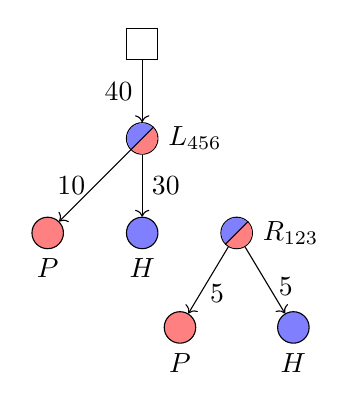
\begin{tikzpicture}[y=1.2cm, x=1.2cm]
      \node[sqadj] (adj) at (0, 0) {};
      \node[circAB, label=right:$L_{456}$] (L) at (0, -1) {};
      \node[circA, label=below:$P$] (A) at (-1, -2) {};
      \node[circB, label=below:$H$] (B) at (0, -2) {};
      \node[circAB, label=right:$R_{123}$] (chi) at (1, -2) {};
      \draw[->] (adj) edge node[midway, left] { $40$ } (L);
      \draw[->] (L) edge node[midway, left] { $10$ } (A);
      \draw[->] (L) edge node[midway, right] { $30$ } (B);

      \node[circA, label=below:$P$] (chiA) at (0.4, -3) {};
      \node[circB, label=below:$H$] (chiB) at (1.6, -3) {};

      \draw[->] (chi) edge node[pos=0.7, right] { $5$ } (chiA);
      \draw[->] (chi) edge node[pos=0.6, right] { $5$ } (chiB);
    \end{tikzpicture}
  };

  \node[right=of s1] (s2) {
    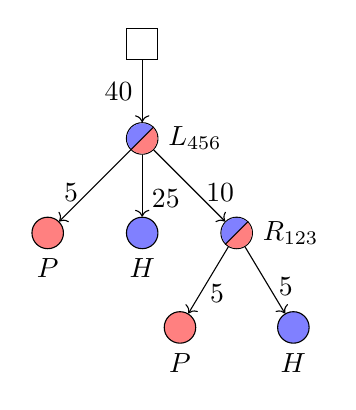
\begin{tikzpicture}[y=1.2cm, x=1.2cm]
      \node[sqadj] (adj) at (0, 0) {};
      \node[circAB, label=right:$L_{456}$] (L) at (0, -1) {};
      \node[circA, label=below:$P$] (A) at (-1, -2) {};
      \node[circB, label=below:$H$] (B) at (0, -2) {};
      \node[circAB, label=right:$R_{123}$] (chi) at (1, -2) {};
      \draw[->] (adj) edge node[midway, left] { $40$ } (L);

      \draw[->] (L) edge node[pos=0.6, left] { $5$ } (A);
      \draw[->] (L) edge node[pos=0.7, right] { $25$ } (B);
      \draw[->] (L) edge node[pos=0.6, right] { $10$ } (chi);

      \node[circA, label=below:$P$] (chiA) at (0.4, -3) {};
      \node[circB, label=below:$H$] (chiB) at (1.6, -3) {};

      \draw[->] (chi) edge node[pos=0.7, right] { $5$ } (chiA);
      \draw[->] (chi) edge node[pos=0.6, right] { $5$ } (chiB);
    \end{tikzpicture}
  };

  \node[right=of s2] (s3) {
    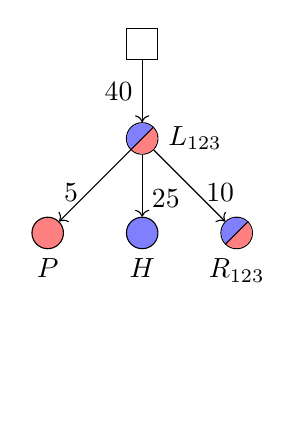
\begin{tikzpicture}[y=1.2cm, x=1.2cm]
      \node[sqadj] (adj) at (0, 0) {};
      \node[circAB, label=right:$L_{123}$] (L) at (0, -1) {};
      \node[circA, label=below:$P$] (A) at (-1, -2) {};
      \node[circB, label=below:$H$] (B) at (0, -2) {};
      \node[circAB, label=below:$R_{123}$] (chi) at (1, -2) {};
      \node[circle, draw=none, label=below:\strut] at (0, -3) {}; %ghost node for alignment%
      \draw[->] (adj) edge node[midway, left] { $40$ } (L);
      \draw[->] (L) edge node[pos=0.6, left] { $5$ } (A);
      \draw[->] (L) edge node[pos=0.7, right] { $25$ } (B);
      \draw[->] (L) edge node[pos=0.6, right] { $10$ } (chi);
    \end{tikzpicture}
  };

  \begin{scope}[shorten <=1cm, shorten >=1.4cm, -{Latex[length=2mm]}]
    \node (level) at (0, 0.8) {};
    \draw (s0 |- level) to (s1 |- level);
    \draw (s1 |- level) to (s2 |- level);
    \draw (s2 |- level) to (s3 |- level);
  \end{scope}
\end{tikzpicture}



\begin{tikzpicture}[x=0.7cm]
  \node (pic1) at (0, 0) {
    \begin{tikzpicture}
      \node[sqadj] (adj1) at (0, 1) {};
      \node[circAB, label=below:$TTT$] (L1) at (0, 0) {};

      \draw[->] (adj1) edge node[midway, left] { 5 } (L1);
    \end{tikzpicture}
  };

  \node (pic2) at (3, 0) {
    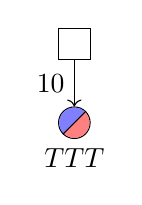
\begin{tikzpicture}
      \node[sqadj] (adj1) at (0, 1) {};
      \node[circAB, label=below:$TTT$] (L1) at (0, 0) {};

      \draw[->] (adj1) edge node[midway, left] { 10 } (L1);
    \end{tikzpicture}
  };

  \node (pic3) at (7, 0) {
    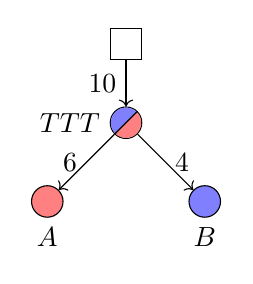
\begin{tikzpicture}
      \node[sqadj] (adj1) at (0, 1) {};
      \node[circAB, label=left:$TTT$] (L1) at (0, 0) {};
      \node[circA, label=below:$A$] (A1) at (-1, -1) {};
      \node[circB, label=below:$B$] (B1) at (1, -1) {};

      \draw[->] (adj1) edge node[midway, left] { 10 } (L1);
      \draw[->] (L1) edge node[midway, left] { 6 } (A1);
      \draw[->] (L1) edge node[midway, right] { 4 } (B1);
    \end{tikzpicture}
  };

  \node (pic4) at (11, 0) {
    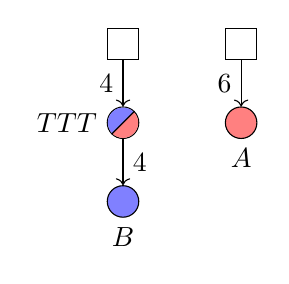
\begin{tikzpicture}
      \node[sqadj] (adj1) at (0, 1) {};
      \node[circAB, label=left:$TTT$] (L1) at (0, 0) {};
      \node[circB, label=below:$B$] (B1) at (0, -1) {};

      \node[sqadj] (adj2) at (1.5, 1) {};
      \node[circA, label=below:$A$] (A1) at (1.5, 0) {};

      \draw[->] (adj1) edge node[midway, left] { 4 } (L1);
      \draw[->] (adj2) edge node[midway, left] { 6 } (A1);
      \draw[->] (L1) edge node[midway, right] { 4 } (B1);
    \end{tikzpicture}
  };

  \node (pic5) at (15, 0) {
    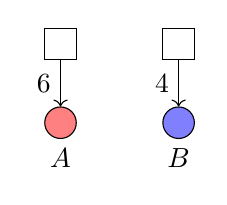
\begin{tikzpicture}
      \node[sqadj] (adj2) at (0, 1) {};
      \node[circA, label=below:$A$] (A1) at (0, 0) {};

      \node[sqadj] (adj1) at (1.5, 1) {};
      \node[circB, label=below:$B$] (B1) at (1.5, 0) {};

      \draw[->] (adj2) edge node[midway, left] { 6 } (A1);
      \draw[->] (adj1) edge node[midway, left] { 4 } (B1);
    \end{tikzpicture}
  };
\end{tikzpicture}



\begin{tikzpicture}[x=0.7cm]
  \node (pic1) at (0, 0) {
    \begin{tikzpicture}
      \node[sqadj] (adj1) at (0, 1) {};
      \node[circAB, label=left:$L_1$] (L1) at (0, 0) {};
      \node[circA] (A1) at (-1, -1) {};
      \node[circB] (B1) at (1, -1) {};

      \node[sqadj] (adj2) at (4, 1) {};
      \node[circAB, label=left:$L_2$] (L2) at (4, 0) {};
      \node[circA] (A2) at (3, -1) {};
      \node[circB] (B2) at (5, -1) {};

      \node[circAB, label=left:$L_3$] (L3) at (2, -2) {};
      \node[circA] (A3) at (1, -3) {};
      \node[circB] (B3) at (3, -3) {};

      \begin{scope}[->]
        \draw (adj1) edge node[midway, left] { 10 } (L1);
        \draw (L1) edge node[midway, left] { 5 } (A1);
        \draw (L1) edge node[midway, right] { 5 } (B1);

        \draw (adj2) edge node[midway, left] { 10 } (L2);
        \draw (L2) edge node[midway, left] { 5 } (A2);
        \draw (L2) edge node[midway, right] { 5 } (B2);

        \draw (L3) edge node[midway, left] { 10 } (A3);
        \draw (L3) edge node[midway, right] { 10 } (B3);
      \end{scope}
    \end{tikzpicture}
  };


  \node (pic2) at (8, 0) {
    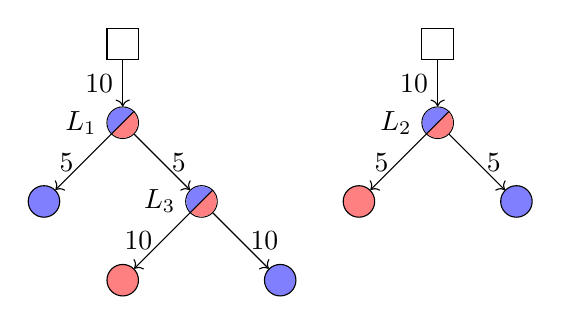
\begin{tikzpicture}
      \node[sqadj] (adj1) at (0, 1) {};
      \node[circAB, label=left:$L_1$] (L1) at (0, 0) {};
      \node[circB] (B1) at (-1, -1) {};

      \node[sqadj] (adj2) at (4, 1) {};
      \node[circAB, label=left:$L_2$] (L2) at (4, 0) {};
      \node[circA] (A2) at (3, -1) {};
      \node[circB] (B2) at (5, -1) {};

      \node[circAB, label=left:$L_3$] (L3) at (1, -1) {};
      \node[circA] (A3) at (0, -2) {};
      \node[circB] (B3) at (2, -2) {};

      \begin{scope}[->]
        \draw (adj1) edge node[midway, left] { 10 } (L1);
        \draw (L1) edge node[midway, left] { 5 } (B1);

        \draw (adj2) edge node[midway, left] { 10 } (L2);
        \draw (L2) edge node[midway, left] { 5 } (A2);
        \draw (L2) edge node[midway, right] { 5 } (B2);

        \draw (L1) edge node[midway, right] { 5 } (L3);

        \draw (L3) edge node[midway, left] { 10 } (A3);
        \draw (L3) edge node[midway, right] { 10 } (B3);
      \end{scope}
    \end{tikzpicture}
  };

  \node (pic3) at (16, 0) {
    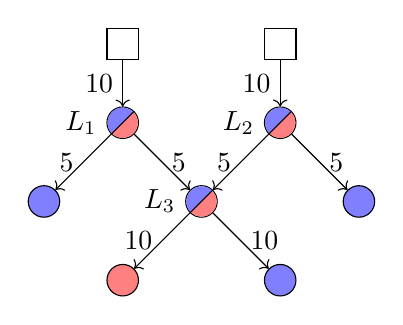
\begin{tikzpicture}
      \node[sqadj] (adj1) at (0, 1) {};
      \node[circAB, label=left:$L_1$] (L1) at (0, 0) {};
      \node[circB] (B1) at (-1, -1) {};

      \node[sqadj] (adj2) at (2, 1) {};
      \node[circAB, label=left:$L_2$] (L2) at (2, 0) {};
      \node[circB] (B2) at (3, -1) {};

      \node[circAB, label=left:$L_3$] (L3) at (1, -1) {};
      \node[circA] (A3) at (0, -2) {};
      \node[circB] (B3) at (2, -2) {};

      \begin{scope}[->]
        \draw (adj1) edge node[midway, left] { 10 } (L1);
        \draw (L1) edge node[midway, left] { 5 } (B1);

        \draw (adj2) edge node[midway, left] { 10 } (L2);
        \draw (L2) edge node[midway, right] { 5 } (B2);

        \draw (L2) edge node[midway, left] { 5 } (L3);
        \draw (L1) edge node[midway, right] { 5 } (L3);

        \draw (L3) edge node[midway, left] { 10 } (A3);
        \draw (L3) edge node[midway, right] { 10 } (B3);
      \end{scope}
    \end{tikzpicture}
  };

  \node (pic4) at (0, -6) {
    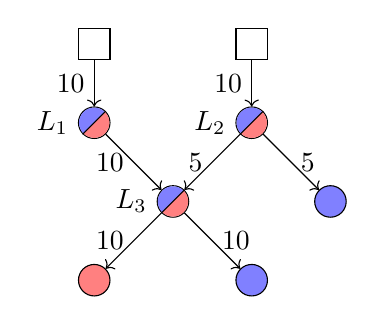
\begin{tikzpicture}
      \node[sqadj] (adj1) at (0, 1) {};
      \node[circAB, label=left:$L_1$] (L1) at (0, 0) {};

      \node[sqadj] (adj2) at (2, 1) {};
      \node[circAB, label=left:$L_2$] (L2) at (2, 0) {};
      \node[circB] (B2) at (3, -1) {};

      \node[circAB, label=left:$L_3$] (L3) at (1, -1) {};
      \node[circA] (A3) at (0, -2) {};
      \node[circB] (B3) at (2, -2) {};

      \begin{scope}[->]
        \draw (adj1) edge node[midway, left] { 10 } (L1);

        \draw (adj2) edge node[midway, left] { 10 } (L2);
        \draw (L2) edge node[midway, right] { 5 } (B2);

        \draw (L2) edge node[midway, left] { 5 } (L3);
        \draw (L1) edge node[midway, left] { 10 } (L3);

        \draw (L3) edge node[midway, left] { 10 } (A3);
        \draw (L3) edge node[midway, right] { 10 } (B3);
      \end{scope}
    \end{tikzpicture}
  };

  \node (pic5) at (8, -6) {
    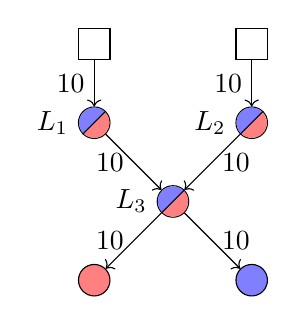
\begin{tikzpicture}
      \node[sqadj] (adj1) at (0, 1) {};
      \node[circAB, label=left:$L_1$] (L1) at (0, 0) {};

      \node[sqadj] (adj2) at (2, 1) {};
      \node[circAB, label=left:$L_2$] (L2) at (2, 0) {};

      \node[circAB, label=left:$L_3$] (L3) at (1, -1) {};
      \node[circA] (A3) at (0, -2) {};
      \node[circB] (B3) at (2, -2) {};

      \begin{scope}[->]
        \draw (adj1) edge node[midway, left] { 10 } (L1);

        \draw (adj2) edge node[midway, left] { 10 } (L2);

        \draw (L2) edge node[midway, right] { 10 } (L3);
        \draw (L1) edge node[midway, left] { 10 } (L3);

        \draw (L3) edge node[midway, left] { 10 } (A3);
        \draw (L3) edge node[midway, right] { 10 } (B3);
      \end{scope}
    \end{tikzpicture}
  };

  \node (pic6) at (15, -6) {
    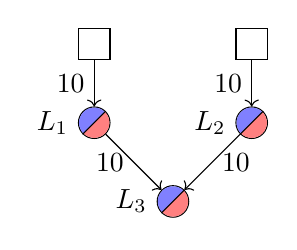
\begin{tikzpicture}
      \node[sqadj] (adj1) at (0, 1) {};
      \node[circAB, label=left:$L_1$] (L1) at (0, 0) {};

      \node[sqadj] (adj2) at (2, 1) {};
      \node[circAB, label=left:$L_2$] (L2) at (2, 0) {};

      \node[circAB, label=left:$L_3$] (L3) at (1, -1) {};

      \begin{scope}[->]
        \draw (adj1) edge node[midway, left] { 10 } (L1);

        \draw (adj2) edge node[midway, left] { 10 } (L2);

        \draw (L2) edge node[midway, right] { 10 } (L3);
        \draw (L1) edge node[midway, left] { 10 } (L3);

      \end{scope}
    \end{tikzpicture}
  };
\end{tikzpicture}



%----


\begin{tikzpicture}[x=0.7cm]
  \node (diag0) at (5, -1) {
    \begin{tikzpicture}[y=0.8cm, x=1.2cm]
      \node[sqadj] (adj) at (1, 0) {};
      \node[semicircle, draw, label=right:$G$] (g) at (1, -1) {};
      \node[semicircle, draw, rotate=180, label=355:$L$] (l) at (1,-2) {};
      \node[circB, label=below:$B$] (b) at (0.58, -3) {};
      \node[circA, label=below:$A$] (a) at (1.42, -3) {};


      \draw[-] (g.220) to[out=270, in=90] (l.220);
      \draw[-] (g.320) to[out=270, in=90] (l.320);

      \draw[->] (adj) edge node[midway, left] { $10$ } (g);
      \draw[->] (l) edge node[midway, left] { $10$ } (b);
      \draw[->] (l) edge node[midway, right] { $10$ } (a);
    \end{tikzpicture}
  };


  \node (diag1) at (10, -1) {
    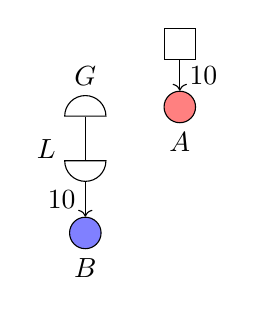
\begin{tikzpicture}[y=0.8cm, x=1.2cm]
      \node[semicircle, draw, label=above:$G$] (g) at (1, -1) {};
      \node[semicircle, draw, rotate=180, label=355:$L$] (l) at (1,-2) {};
      \node[circB, label=below:$B$] (b) at (1, -3) {};

      \draw[-] (g.270) to[out=270, in=90] (l.270);

      \draw[->] (l) edge node[midway, left] { $10$ } (b);

      \node[sqadj] (a2) at (2, 0) {};
      \node[circA, label=below:$A$] (pa) at (2, -1) {};
      \draw[->] (a2) edge node[midway, right] { $10$ } (pa);
    \end{tikzpicture}
  };
\end{tikzpicture}



\end{document}
